%!TEX root = ../main.tex
% chktex-file 46
\chapter{Evaluation}%
\label{sec:eval}

In \cref{sec:ltag} the relation between \ac{lta} and existing \ac{gcr} approaches was formally analyzed.
There we saw that the \ac{lta} formulations of existing approaches mostly use static decomposition functions, e.g.\ \ac{bfs} subtree decompositions.
Motivated by the idea of dynamically learning decompositions via edge filters, we then proposed the novel 2-\acs{wl}-\acs{gnn} in \cref{sec:ltd}.
The ides presented in both chapters will now be empirically evaluated.
Do to so we differentiate between two mostly independent evaluation aspects:
\begin{enumerate}[label={\textbf{\arabic*.}}]
	\item \textbf{Evaluation of 2-\acs{wl}-\acsp{gnn}:}
		Even though it was motivated by \ac{lta}, a 2-\acs{wl}-\acs{gnn} is not generally more ``\acs{lta}-like'' than other approaches.
		Nonetheless, due to the theoretical advantages described in \cref{sec:ltd:wl2gnn:properties} it is an interesting approach independently from its potential applications in \ac{lta} (see \cref{sec:ltd:edge-filter}).
		Thus the first aspect of our evaluation is to compare 2-\acs{wl}-\acsp{gnn} with the other previously described \ac{gcr} methods in a general non-\acs{lta} fashion, i.e.\ with an added \ac{mlp} after the pooling layer since this is how \acp{gnn} are typically evaluated in other works.
	\item \textbf{Evaluation of the \ac{lta} assumption:}
		We previously described that a given domain problem satisfies the \ac{lta} assumption if its solutions can be described by an \ac{lta} formulation (see \cfullref{defn:ltag:lta-assumption}).
		The inherent bias of an \acs{lta}-like model towards such \ac{lta} formulations could potentially increase its generalization performance compared to more general non-\acs{lta} models.
		Therefore the second aspect of our evaluation is to compare the performance of the previously described \acs{lta}-like methods with that of non-\acs{lta} approaches on datasets from multiple problem domains.
\end{enumerate}
This chapter will tackle those two aspects in four steps:
\begin{enumerate*}[label={\circled{\small\arabic*}}]
	\item We begin by describing the experimental setup used to obtain the evaluation results in \cref{sec:eval:setup}.
	\item We then present results on synthetically generated data in \cref{sec:eval:synthetic}.
	 	There we will illustrate the higher expressive power of 2-\acs{wl}-\acsp{gnn} when compared to other \ac{gcr} approaches which confirms the theoretical results from \cref{sec:ltd:wl2gnn:properties}.
	\item Then evaluation results on real-world datasets are described in \cref{sec:eval:real}.
		There we will see how 2-\acs{wl}-\acsp{gnn} compare to other \acp{gnn} in practice as well as how \acs{lta}-like models compare to non-\acs{lta} model.
	\item Finally, \cref{sec:eval:lta} looks at the synthetic and real-world results from an \ac{lta} perspective.
		There we will see how the predictive performance of an \acs{lta}-like model relates to the size and locality of its constituents.
\end{enumerate*}

\section{Experimental Setup}%
\label{sec:eval:setup}

In our experimental evaluation we focus on two types of learners:
\acp{svm} using graph kernels and \acp{gcnn}.
We evaluate those learners by comparing their test accuracies on multiple binary classification problems.
To obtain those accuracies we follow the graph classification benchmarking framework recently proposed by \citet{Errica2020}.
Their benchmarking framework is motivated by the observation that most recent publications in the field of \acp{gnn} do not provide reproducible results.
To tackle this issue they evaluated multiple state-of-the-art methods using a unified model selection procedure:\\
{\setlength{\intextsep}{0pt}%
\begin{minipage}[t]{0.55\linewidth-1em}
	\begin{algorithm}[H]
		\caption{$k$-fold Model Assessment}\label{algo:eval:assessment}
		\begin{algorithmic}[1]
			\State{\textbf{Input:} Dataset $\mathcal{D}$, configurations $\Theta$}
			\State{Split $\mathcal{D}$ into $k$ folds $F_1, \dots, F_{k}$}
			\For{$i \leftarrow 1, \dots, k$}
				\State{$\mathcal{D}_{\mathrm{train/val}}, \mathcal{D}_{\mathrm{test}} \leftarrow \left( \bigcup_{j \neq i} F_{j} \right), F_i$}
				\State{Split $\mathcal{D}_{\mathrm{train/val}}$ into $\mathcal{D}_{\mathrm{train}}, \mathcal{D}_{\mathrm{val}}$}
				\State{$\theta_{\mathrm{best}} \leftarrow \Call{Select}{\mathcal{D}_{\mathrm{train}}, \mathcal{D}_{\mathrm{val}}, \Theta}$}
				\For{$r \leftarrow 1, \dots, R$}
					\State{$h_{i,r} \leftarrow \Call{Train}{\mathcal{D}_{\mathrm{train}}, \theta_{\mathrm{best}}}$}
					\State{$\mathit{acc}_{i,r} \leftarrow \Call{Eval}{h_{i,r}, \mathcal{D}_{\mathrm{test}}}$}
				\EndFor{}
				\State{$\mathit{acc}_{i} \leftarrow \mean_{r \in [R]}{\mathit{acc}_{i,r}}$}
			\EndFor{}
			\State{\Return{$\mean_{i \in [k]} \mathit{acc}_i, \mathrm{stddev}_{i \in [k]}\, \mathit{acc}_i$}}
		\end{algorithmic}
	\end{algorithm}
\end{minipage}\hspace*{1em}%
\begin{minipage}[t]{0.45\linewidth}
	\begin{algorithm}[H]
		\caption{Model Selection}\label{algo:eval:selection}
		\begin{algorithmic}[1]
			\Function{Select}{$\mathcal{D}_{\mathrm{train}}, \mathcal{D}_{\mathrm{val}}, \Theta$}
			\ForAll{$\theta \in \Theta$}
				\State{$h_{\theta} \leftarrow \Call{Train}{\mathcal{D}_{\mathrm{train}}, \theta}$}
				\State{$\mathit{acc}_{\theta} \leftarrow \Call{Eval}{h_{\theta}, \mathcal{D}_{\mathrm{val}}}$}
			\EndFor{}
			\State{$\theta_{\mathrm{best}} \leftarrow \arg\max_{\theta \in \Theta}{\mathit{acc}_{\theta}}$}
			\State{\Return{$\theta_{\mathrm{best}}$}}
			\EndFunction{}
		\end{algorithmic}
	\end{algorithm}
\end{minipage}}

We base our evaluations on this assessment strategy with $k = 10$ folds and $r = 3$ repeats per fold to smooth out differences caused by random weight initializations.
For each dataset the same folds are used across the evaluated models; class proportions are preserved within each fold by using stratified splits.
To keep the total runtime of the experiments feasible, a single 90\%/10\% holdout split into training and validation data is used instead of cross-validation.
To train models that require gradient-based optimization, we use the well-known Adam optimizer~\cite{Kingma2015} and the standard binary crossentropy loss.
In all experiments, training is performed with an early stopping condition which cancels the optimization if there is no improvement to the validation loss for more than $p$ epochs.
The patience period $p$ is part of the hyperparameter configurations $\theta \in \Theta$.

Using this assessment strategy we evaluate \acp{svm} with the following graph kernels:
\begin{enumerate}[label={\textbf{\arabic*.}},itemsep=2pt,parsep=2pt]
	\item \textbf{\ac{wl} subtree kernel (\acs{wl}\textsubscript{ST})} with the iteration counts $T \in \{ 1,2,3,4,5 \}$ to evaluate the influence of the depth of \ac{bfs} subtrees which span \ac{lta} constituents.
	\item \textbf{\ac{wl} shortest path kernel (\acs{wl}\textsubscript{SP})} with the iteration count $T = 3$.
	\item \textbf{2-LWL kernel} with the iteration count $T = 3$.
	\item \textbf{2-GWL kernel} with the iteration count $T = 3$.
\end{enumerate}
The gram matrices of the \acs{wl}\textsubscript{ST} and \acs{wl}\textsubscript{SP} kernels are computed via the \citetitle{GK} library~\cite{Siglidis2018}\cite{GK}.
For the gram matrices of the two dimensional \ac{wl} kernels we use a modified version\footnote{\url{https://github.com/Cortys/glocalwl}} of the reference implementation provided by \citet{Morris2017}.
To train \acp{svm} with those kernels, \citetitle{SKL}~\cite{Pedregosa2011}\cite{SKL} is used.
For the evaluation of \acp{gcnn} we selected the following methods:
\begin{enumerate}[label={\textbf{\arabic*.}},itemsep=2pt,parsep=2pt]
	\item \textbf{Structure unaware baseline:}
		\citet{Errica2020} describe a simple model which simply applies a standard \ac{mlp} to each individual vertex feature vector, then sums up the resulting feature vectors and applies another \ac{mlp} to the vector sum.
		This approach does not use any structural information and therefore serves as a baseline to detect whether a \ac{gnn} is able to exploit graph structure.
	\item \textbf{\ac{gin}} is evaluated as described by \citet{Xu2018}, i.e.\ with a sum pooling layer and an appended \ac{mlp} to produce the final prediction.
	\item \textbf{2-\acs{gnn}} is evaluated with both a static $\mean$ pooling layer and with \ac{sampool} (see \cfullref{defn:ltag:sam-pool}).
		After the pooling layer a \ac{mlp} is used to produce the final prediction.
	\item \textbf{2-\acs{wl}-\ac{gnn}} \textit{(our method)} is also evaluated with $\mean$ pooling and \ac{sampool}, just like 2-\ac{gnn}.
		To test the \ac{lta} assumption we evaluate 2-\acs{wl}-\acs{gnn} in an \acs{lta}-like configuration and in the standard non-\acs{lta} configuration.
		The \acs{lta}-like configuration uses a stack of 2-\acs{wl} convolutions that produce a local prediction $y_{ij} \in [0, 1]$ for each edge $e_{ij}$ instead of a local feature vector $z_{ij} \in \mathbb{R}^{d^{(T)}}$ and it does not have an \ac{mlp} after the pooling/aggregation layer.
\end{enumerate}
The baseline and \ac{gin} results are obtained using the PyTorch-based implementation provided by \citet{Errica2020}.
For both 2-\acs{gnn} and 2-\acs{wl}-\ac{gnn} a custom TensorFlow-based implementation is used.
The code for all conducted experiments as well as the used dataset splits are available GitHub\footnote{\url{https://github.com/Cortys/master-thesis}}.
The evaluated hyperparameter configurations $\Theta$ are described in \cref{sec:appendix:config-grid}.

\section{Evaluation on Synthetic Data}%
\label{sec:eval:synthetic}

We begin with an evaluation of graph kernels and \acp{gnn} on a synthetic binary classification dataset which demonstrates the potential advantages of a higher dimensional \ac{wl} method such as the proposed 2-\acs{wl}-\acs{gnn}.
To determine the classes of the graphs in this dataset, a learner has to solve the so-called \textit{unicolored triangle detection} problem:
Given a graph $G$ with vertices that are colored as either $l_G[v] = \colorlabel{t_blue}{A}$ or as $l_G[v] = \colorlabel{t_red}{B}$, the learner has to find the unique triangle $(v_i, v_j, v_k)$ in $G$ for which $l_G[v_i] = l_G[v_j] = l_G[v_k]$. % chktex 25
The class of $G$ is then determined by the color of the vertices $(v_i, v_j, v_k)$.

Based on this problem we generated a synthetic triangle detection dataset.
It contains randomly generated graphs with varying vertex counts and vertex color proportions (see \cref{sec:appendix:ds-stats} for a more detailed description).
We use this dataset to evaluate whether a learner is able to ignore varying amounts of noisy random structure and focus on relevant local substructures, in this case unicolored triangles.
For the evaluation of 2-\acs{wl}-\acsp{gnn}, the neighborhood radius $r = 2$ is used.
\begin{table}[t]
	\caption{Mean accuracies and standard deviations on the triangle detection dataset.}\label{tbl:eval:synthetic}
	\centering
	\csvreader[
		tabular={clrrr},
		separator=semicolon,
		table head={%
			& \multicolumn{2}{l}{Model (Iterations/Pooling)} & \multicolumn{1}{c}{Train} & \multicolumn{1}{c}{Test} \\\toprule%
		},
		table foot=\bottomrule,
		late after line=\ifthenelse{\equal{\id}{9}}{\\\midrule}{\\},
		head to column names,
		filter=\equal{\isDefault}{1}\or\equal{\id}{4}
	]{data/results.csv}{}{%
		\ifthenelse{\equal{\id}{0}}{\multirow{6}{*}[0em]{\rotatebox[origin=c]{90}{\small\textsc{Kernel}}}}{}%
		\ifthenelse{\equal{\id}{9}}{\multirow{8}{*}[0em]{\rotatebox[origin=c]{90}{\small\textsc{\ac{gnn}}}}}{} &%
		\textbf{\ifthenelse{\equal{\isLta}{1}}{\textcolor{t_darkgreen}{\model*}}{\model\ifthenelse{\equal{\model}{2-WL-GNN}}{\phantom{*}}{}}} ($\params$) & \ifthenelse{\equal{\isLta}{1}}{\badgeboxinline[t_green]{\scriptsize \acs*{lta}-like}}{} &%
		\evalres[\and\not\equal{\id}{8}]{\triangleBestTrain}{\triangleTrainMean}{\triangleTrainStd} & \evalres{\triangleBestTest}{\triangleTestMean}{\triangleTestStd}%
	}
\end{table}
\begin{figure}[t]
	\centering
	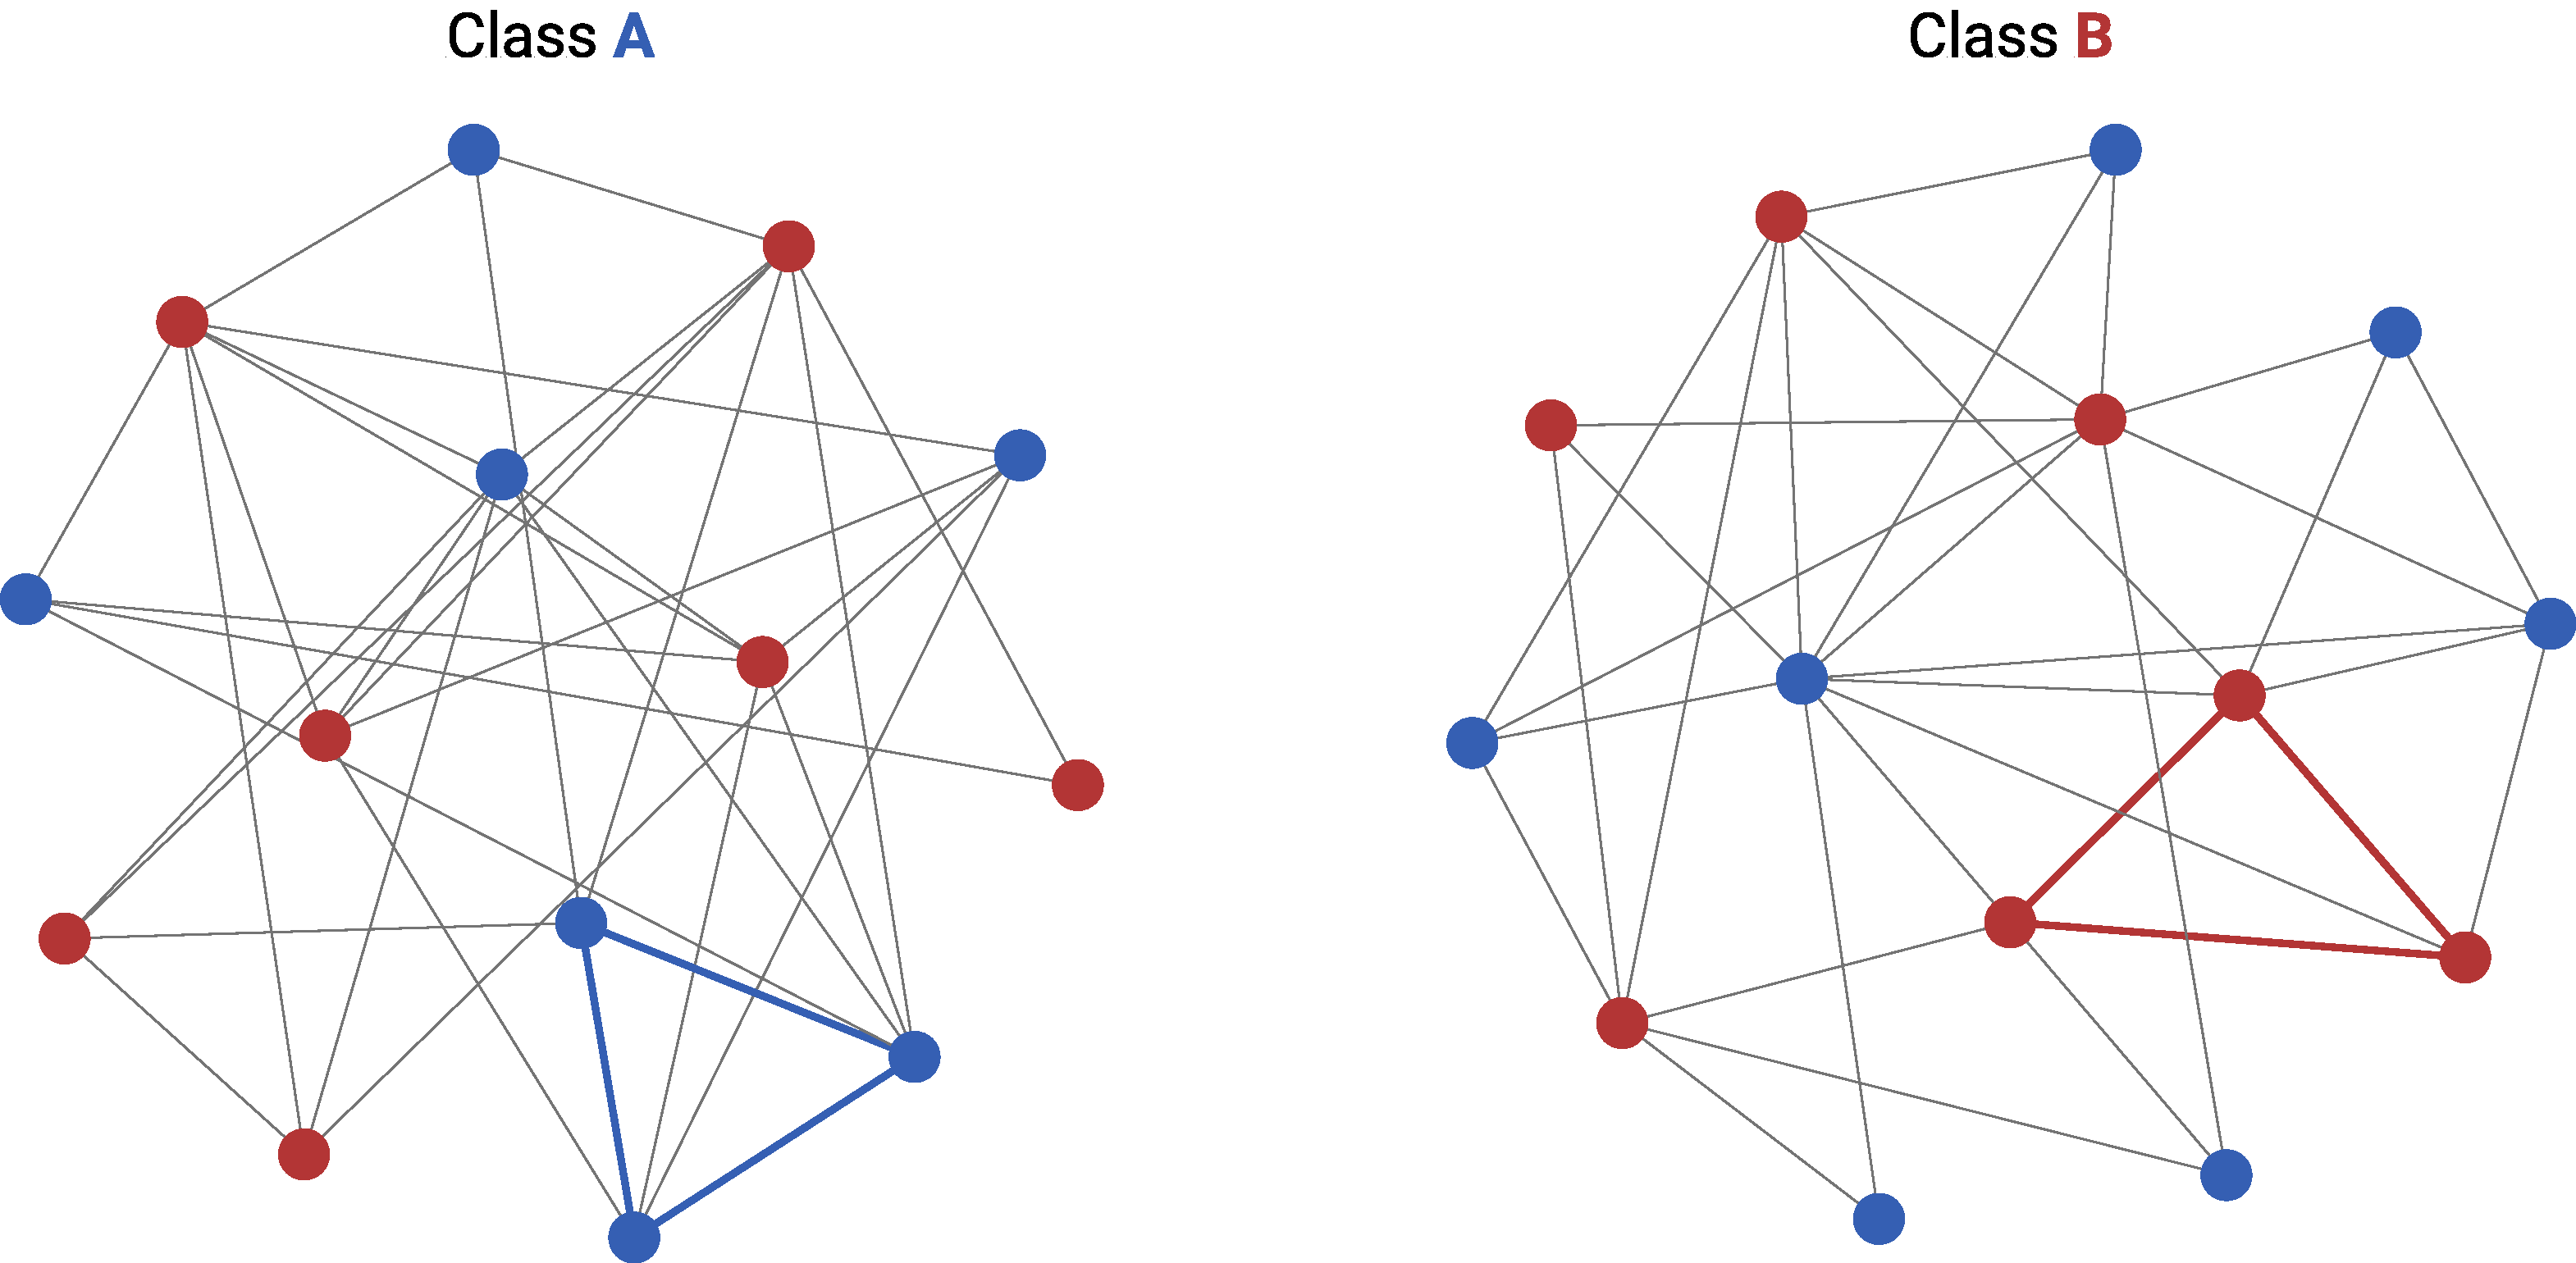
\includegraphics[width=0.7\linewidth]{gfx/evaluation/triangle-problem.pdf}
	\caption[Two example graphs from the triangle detection dataset.]{
		Two examples from the triangle detection dataset.
		The unique unicolored triangle, which has to be detected by the learners, is highlighted in both graphs.
	}\label{fig:evaluation:triangle-problem}
\end{figure}

Looking at the results in \cref{tbl:eval:synthetic}, it can be seen that the structure unaware baseline method is completely unable to detect triangles, as expected.
The structure aware learners on the other hand all perform better than random guessing and are in fact mostly able to fit the training data perfectly.
This shows that all generated graphs are 1-\acs{wl} distinguishable; the \ac{wl} subtree kernel, for example, can simply memorize the training graphs via their unique 1-\acs{wl} color distribution after $T = 5$ refinement steps.

However, the ability to distinguish training graphs is not sufficient to also classify previously unseen graphs correctly.
Since 1-\acs{wl} cannot detect triangles, all 1-\acs{wl} bounded approaches (\acs{wl}\textsubscript{ST}, \acs{wl}\textsubscript{SP}, Baseline, \acs{gin}) are therefore unable to generalize, as can be seen in their test accuracies.
The fact that they perform better than random guessing can be explained by the following proxy indicator:
The presence of an \colorlabel{t_blue}{A}-colored triangle in a graph $G$ implies that there is a local region with a slightly higher density of \colorlabel{t_blue}{A}-colored vertices than in a \colorlabel{t_red}{B}-colored graph $H$ with the same vertex color proportions.
This local color density difference is already detectable in the depth-1 \acs{bfs} subtrees used by 1-\acs{wl} after a single refinement step; this explains why \acs{wl}\textsubscript{ST} performs similarly for $T = 1$ and $T = 5$.

Let us now take a look at the 2-\acs{wl} inspired kernels: 2-LWL and 2-GWL.\@
Interestingly both kernels do not appear to generalize better the 1-\acs{wl} bounded methods;
we explain this by the fairly small size of the triangle detection dataset (228 graphs).
Even though both kernels embed graphs into a space with dimensions that indicate the presence of a unicolored triangle (see \cfullref{prop:related:wl2-cycle-count}), there are many of those triangle-indicating embedding dimensions s.t.\ the indicating dimensions found in a given training split might not overlap with those in the test split.

Looking at the 2-\acs{wl} inspired \acp{gnn} (2-\acs{gnn}, 2-\acs{wl}-\acs{gnn}), we find that the proposed 2-\acs{wl}-\acs{gnn} significantly outperforms all other evaluated methods which confirms our theoretical results from \cref{sec:ltd:wl2gnn:properties}.
We evaluated 2-\acs{wl}-\acsp{gnn} in an \acs{lta}-like configuration without a final \ac{mlp} and in a non-\acs{lta} configuration with an \ac{mlp} after the pooling layer.
Comparing both configurations, we see that the \acs{lta}-variant has a worse generalization performance despite the fact that the triangle detection problem fits well into the \ac{lta} framework:
\begin{enumerate*}[label={\circled{\small\arabic*}}]
	\item Decomposition corresponds to finding a single unicolored triangle constituent,
	\item local evaluation then corresponds to checking the color of the triangle constituent and
	\item aggregation is trivial since there is only one constituent.
\end{enumerate*}

However, as we saw in the \ac{lta} formulation of \acp{gcnn} (see \cfullref{thm:ltag:gcnn-ltag-formulation}), a 2-\acs{wl}-\acs{gnn} does not actually learn to decompose a graph into unicolored triangle constituents but uses subtree constituents instead.
Further investigations are required to determine to which extent the worse performance of the \acs{lta}-like configuration is caused by this static decomposition strategy and whether a more dynamic solution to the \acf{ltd} problem could improve the performance (e.g.\ via the edge filtering idea described in \cref{sec:ltd:edge-filter}).

Finally, if we look at the two evaluated pooling layers, static $\mean$ pooling and \ac{sampool}, we see that the attention mechanism of the latter significantly improves the generalization performance of both 2-\acsp{gnn} and 2-\acs{wl}-\acsp{gnn}.
This indicates that \ac{sampool} is successful at filtering out the randomly generated noisy parts of a given graph and putting most attention to the relevant unicolored triangle.

\section{Evaluation on Real-World Data}%
\label{sec:eval:real}

\begin{table}[ht]
	\caption[Mean test accuracies and standard deviations on real-world data.]{
		Mean test accuracies and standard deviations on real-world data.
		\hfill\textcolor{t_darkgreen}{*}\,\badgeboxinline[t_green]{\scriptsize\acs*{lta}-like}
	}\label{tbl:eval:real}
	\centering
	\csvreader[
		tabular={lrrrrr},
		separator=semicolon,
		table head={%
			& %
			\multicolumn{1}{c}{\hyperref[tbl:appendix:diff-nci]{\textbf{NCI1}}} &%
			\multicolumn{1}{c}{\hyperref[tbl:appendix:diff-proteins]{\textbf{PROTEINS}}} &%
			\multicolumn{1}{c}{\hyperref[tbl:appendix:diff-dd]{\textbf{D\&D}}} &%
			\multicolumn{1}{c}{\hyperref[tbl:appendix:diff-reddit]{\textbf{REDDIT}}} &%
			\multicolumn{1}{c}{\hyperref[tbl:appendix:diff-imdb]{\textbf{IMDB}}}%
			\\\toprule%
		},
		table foot=\bottomrule,
		late after line=\ifthenelse{\equal{\id}{9}}{\\\midrule}{\\},
		head to column names,
		filter={\equal{\isDefault}{1}}
	]{data/results.csv}{}{%
		% \ifthenelse{\equal{\id}{0}}{\multirow{5}{*}[0em]{\rotatebox[origin=c]{90}{\small\textsc{Kernel}}}}{}%
		% \ifthenelse{\equal{\id}{9}}{\multirow{8}{*}[0em]{\rotatebox[origin=c]{90}{\small\textsc{\ac{gnn}}}}}{} &%
		\textbf{\ifthenelse{\equal{\isLta}{1}}{\textcolor{t_darkgreen}{\model*}}{\model\ifthenelse{\equal{\model}{2-WL-GNN}}{\phantom{*}}{}}} {\footnotesize($\params$)} &%
		{\small\evalres{\nciBestTest}{\nciTestMean}{\nciTestStd}}&%
		{\small\evalres{\proteinsBestTest}{\proteinsTestMean}{\proteinsTestStd}}&%
		{\small\evalres{\ddBestTest}{\ddTestMean}{\ddTestStd}}&%
		{\small\evalres{\redditBestTest}{\redditTestMean}{\redditTestStd}}&%
		{\small\evalres{\imdbBestTest}{\imdbTestMean}{\imdbTestStd}}%
	}
\end{table}
Since the synthetic triangle detection problem was designed specifically to highlight the advantages of a higher dimensional \ac{wl} method such as 2-\ac{wl}-\acsp{gnn}, we now evaluate the approaches more fairly on five common graph classification benchmark datasets from two different real-world domains:
\begin{enumerate}[label={\textbf{\arabic*.}}]
	\item \textbf{Bioinformatics:}
		The NCI1~\cite{Shervashidze2011}, PROTEINS~\cite{Borgwardt2005a} and D\&D~\cite{Dobson2003} datasets all contain molecular graphs.
		For NCI1 the goal is to predict whether a molecule is effective against certain types of cancer.
		For PROTEINS and D\&D, a learner has to determine whether a given protein molecule is an enzyme.
	\item \textbf{Social networks:}
		The REDDIT and IMDB datasets~\cite{Yanardag2015} contain graphs representing the relations between users in online discussions and movie actors respectively.
		For REDDIT the type of a community has to be predicted based on a discussion thread; for IMDB the goal is to determine movie genres.
\end{enumerate}
A more detailed description of the evaluated datasets can be found in \cref{sec:appendix:ds-stats}.
\Cref{tbl:eval:real} shows our evaluation results\footnote{
	Note that, for the NCI1, PROTEINS and D\&D datasets we used different training/test splits than those originally used by \citet{Errica2020}.
	The reason for this is that the original splits were only published after our evaluations of those datasets had already been completed.
	For REDDIT and IMDB however, we used the same splits.
}.
For the evaluation of 2-\acs{wl}-\acsp{gnn}, different neighborhood radii were used for each dataset.
In the order of the columns in the table above, the results were obtained with the radii $r = 8$, $5$, $2$, $1$ and $4$ respectively.

If we compare the real-world results with those for the synthetic triangle detection dataset, we do no longer observe the clear advantage of 2-\acs{wl}-\acsp{gnn} over the other approaches.
This indicates that the theoretical advantages of 2-\acs{wl} over 1-\acs{wl} are not necessarily relevant for the five evaluated problems.
Nonetheless, the test performance of 2-\acs{wl}-\acsp{gnn} is generally comparable to that of the other state-of-the-art learners with the exception of NCI1,
where by comparable we mean that the performance of the evaluated 2-\acs{wl}-\acs{gnn} models is within the $2\sigma$ confidence interval of the best evaluated model even when compared fold-by-fold (see \cref{sec:appendix:fold-diffs}).

If we look at the enzyme detection problem (PROTEINS and D\&D), we observe that all evaluated approaches appear to be unable to leverage structural information for a significant improvement over the baseline learner (see \cref{tbl:appendix:diff-proteins,{tbl:appendix:diff-dd}}).
In the social network datasets (REDDIT and IMDB) on the other hand, the structure aware methods clearly outperform the baseline (see \cref{tbl:appendix:diff-reddit,tbl:appendix:diff-imdb}).
This confirms the very similar results of \citet{Errica2020}.

Lastly, note that the \acs{lta}-like 2-\acs{wl}-\acs{gnn} configurations either perform significantly worse or roughly similar to their non-\acs{lta} counterparts.
This mirrors our result on the synthetic triangle detection dataset.
Regarding the \acs{lta} assumption (see \cfullref{defn:ltag:lta-assumption}), this is evidence that the decomposition function $\psi$ of 2-\acs{wl}-\acsp{gnn} (see \cfullref{thm:ltag:gcnn-ltag-formulation}) does not produce constituents $c_i \in \psi(G)$ whose local evaluations $f(c_i) \in \mathcal{Y}$ are as indicative of the graph $G$'s class $y \in \mathcal{Y}$ as an arbitrary feature vector $z_i \in \mathbb{R}^{d^{(T)}}$.
This does however not imply, that the evaluated real-world problem domains are generally incompatible with the \ac{lta} assumption.
When considering the results of the \ac{lta}-like \acs{wl}\textsubscript{ST} model, we find that it is mostly comparable with the alternative non-\acs{lta} approaches and, in the case of NCI1, even significantly better.
This shows that local constituent evaluations are in principle suitable for graph classification tasks if the right decomposition, evaluation and aggregation functions are chosen.

\section{Evaluation of \acs*{lta} Constituent Locality}%
\label{sec:eval:lta}

To conclude our evaluation, we now look at the influence of constituent sizes on the test accuracy of \acs{lta}-like models, such as \acs{wl}\textsubscript{ST} and 2-\acs{wl}-\acsp{gnn}.
As described in \cref{sec:ltag:formulation:svm,sec:ltag:formulation:gcnn:conv}, the constituents in the \ac{lta} formulations of both of these models are spanned by \ac{bfs} subtrees of some depth $T$.
Thus, for large $T$, decompositions consist of just the connected components of a graph, i.e.\ they are only partially \acs{lta}-like.

We now analyze for which degree of constituent locality \acs{wl}\textsubscript{ST} and 2-\acs{wl}-\acsp{gnn} perform best by evaluating them using varying tree depths $T$.
For \acs{wl}\textsubscript{ST} we can set $T$ directly via the number of refinement steps.
\Cref{fig:eval:wlst-depths} shows the the accuracies of \acs{wl}\textsubscript{ST} for $T \in \{ 1, \dots, 5 \}$.
On all evaluated datasets, the test accuracy tends to be optimal for some $T \in \{ 1, 2, 3 \}$.%
\newcommand{\wlstDepthPlot}[4][ymin=70, ymax=100, try min ticks=6]{%
\begin{tikzpicture}
	\begin{axis}[
		width=0.35\linewidth,
		height=0.3\linewidth,
		xmin=0.7, xmax=5.3,
		#1,
		label style={font=\tiny},
		tick label style={font=\tiny},
		ymajorgrids,
		ytick style={draw=none},
		ylabel shift=-6pt,
		xlabel shift=-5pt,
		axis line style={gray},
		mark size={1.5pt},
		title={\small #3},
		title style={yshift=-0.5em}
	]
		\begin{scope}[gray]
			\draw[gray, dashed] ({axis cs:#4,0}|-{rel axis cs:0,1}) -- ({axis cs:#4,0}|-{rel axis cs:0,0});
		\end{scope}
		\addplot [color=t_blue, only marks, mark=*]
		plot[error bars/.cd, y dir=both, y explicit]
		table [x=T, y=#2TrainMean, y error=#2TrainStd, col sep=semicolon] {data/wlst_depths.csv};
		\label{pgfplots:eval:wlst-depth:#2-train}
		\addplot [color=t_red, only marks, mark=square*]
		plot[error bars/.cd, y dir=both, y explicit]
		table [x=T, y=#2TestMean, y error=#2TestStd, col sep=semicolon] {data/wlst_depths.csv};
		\label{pgfplots:eval:wlst-depth:#2-test}
	\end{axis}
\end{tikzpicture}} % chktex 31
\begin{figure}[t]
	\centering
	\begin{tabular}{cccc}
		\wlstDepthPlot[ymin=40, ymax=100, try min ticks=6, ylabel={accuracy}]{triangle}{TRIANGLE}{2.3} &
		\wlstDepthPlot{nci}{NCI1}{7} &
		\wlstDepthPlot{proteins}{PROTEINS}{6.1} &
		\multirow{2}{*}[1.5em]{\rotatebox[origin=c]{90}{\scriptsize%
			\ref{pgfplots:eval:wlst-depth:triangle-test}~Test\quad % chktex 2
			\ref{pgfplots:eval:wlst-depth:triangle-train}~Train % chktex 2
		}}\\
		\wlstDepthPlot[ymin=70, ymax=100, try min ticks=6, ylabel={accuracy}, xlabel={no.\ of iterations}]{dd}{D\&D}{10.8} &
		\wlstDepthPlot[ymin=70, ymax=100, try min ticks=6, xlabel={no.\ of iterations}]{reddit}{REDDIT}{4.6} &
		\wlstDepthPlot[ymin=70, ymax=100, try min ticks=6, xlabel={no.\ of iterations}]{imdb}{IMDB}{1.0} &
	\end{tabular}
	\caption[Training and test accuracy of \acs{wl}\textsubscript{ST} for varying iteration counts.]{
		Accuracy of \acs{wl}\textsubscript{ST} for varying iteration counts on the six evaluated datasets from the previous sections.
		The error bars indicate standard deviations.
		The dashed lines indicate the mean graph radius in each dataset (if it is less than $5$).
	}\label{fig:eval:wlst-depths}
\end{figure}
If we compute the mean radii of the graphs in each dataset\footnote{
	The radius of a graph $G$ is defined as $\min_{v \in \mathcal{V}_G} \max_{u \in \mathcal{V}_G} d_{\mathrm{SP}, G}(v, u)$, i.e.\ the distance of the furthest vertex $u$ from the most central vertex $v$ of $G$.
}, we find that they are all larger than $3$, with the exception of the triangle detection and the IMDB dataset (see \cref{tbl:appendix:ds-stats}).
This implies that the best-performing subtree constituents do not span entire connected components but smaller substructures on average.
The REDDIT dataset shows this very clearly; there a subtree must have a depth of at least $5$ in order to span an average graph while the best-performing subtree constituents only have a depth of $T = 2$.
This indicates that the REDDIT community detection problem is better described by small localized constituents than by large non-localized ones.

Let us now look at the constituent locality of 2-\acs{wl}-\acsp{gnn}.
There the depth of constituent subtrees is determined by both the number of convolutional layers and the neighborhood radius $r$.
Just like the iteration count in \acs{wl}\textsubscript{ST}, the number of layers directly determines the number of neighborhood aggregation steps and therefore the subtree sizes.
The neighborhood radius $r$ on the other hand determines how many new edges are present in $G^r$ in comparison to $G$;
when $r$ is increased, the \ac{bfs} subtrees can span larger constituents due to the additional connections.

In addition to its influence on constituent sizes, a higher neighborhood radius also introduces additional feature vectors into the convolved feature matrices $Z^{(t)} \in \mathbb{R}^{\left|\mathcal{E}_{G^r}\right| \times d^{(t)}}$.
As we saw in the proof sketch of 2-\acs{wl}'s cycle counting ability (see \cfullref{prop:related:wl2-cycle-count}), those additional features/colors can carry important structural information about a graph.
